\documentclass[12pt,a4paper]{report}
\usepackage[T2A]{fontenc}
\usepackage[utf8]{inputenc}
\usepackage[russian]{babel}
\usepackage{graphicx, setspace, amsmath}


\usepackage[
top = 1.25cm,
bottom = 2.0cm]{geometry}

\begin{document}
\begin{titlepage}
	\centering
    % HEADER
	{
        \scshape
        Федеральное государственное автономное образовательное учреждение высшего образования
        \par
        \textbf{«Научно-образовательная корпорация ИТМО»}
        \par
        \vspace*{1cm}
        Факультет Программной Инженерии и Компьютерной Техники
        \par
    }
    % LOGO
    \vspace*{0.6cm}
    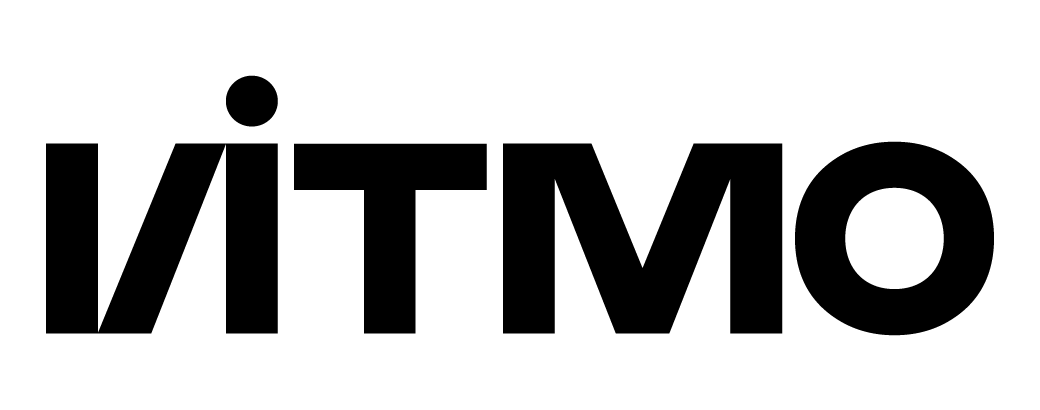
\includegraphics[width=\textwidth]{logo.png}
    % LAB INFO
    {
        \Large
        \textbf{Домашняя работа по представлению чисел в ЭВМ №3}
        \par
        \normalsize
        \vspace*{0.75cm}
        \textbf{Вариант 44}
        \par
    }
    \vfill
    % СREDITS
    \hfill\begin{minipage}{\dimexpr\textwidth-7.8cm}
        \textbf{Выполнил:}\par
        Степанов Арсений Алексеевич\par
        \vspace*{0.15cm}
        \textbf{Группа:}\par
        P3109\par
        \vspace*{0.15cm}
        \textbf{Преподаватель:}\par
        Поляков Владимир Иванович\par
    \end{minipage}
    \vfill
    Санкт-Петербург, \the\year{}г.
\end{titlepage}
\section*{Значения чисел для данного варианта}
\onehalfspacing
$A=32_{10}=00100000_2$\\
$-A=32_{10}=11100000_2$\\
$B=84_{10}=01010100_2$\\
$-B=84_{10}=10101100_2$\\
\section*{Задание №1}
\begin{tabular}{cccc} % Part 1
    \begin{tabular}{c}
        A > 0, B > 0\\
        $
        \large
        \begin{array}{r}
        -
        \begin{array}{r}
        \overset{\normalsize{1}}{\phantom{0}}\overset{\normalsize{1}}{0}0\overset{\normalsize{1}}{1}\overset{\normalsize{1}}{0}\overset{\normalsize{1}}{0}000\\
        01010100\\
        \end{array} \\
        \hline
        \begin{array}{r}
        C_{com}\;\;11001100
        \end{array}\\
        \hline
        \begin{array}{r}
        C_{dir}\;\;00110100
        \end{array}\\
        \end{array}
        $
    \end{tabular} &
    \begin{tabular}{c}
        З.И.\\
        $
        \large
        \begin{array}{r}
        -
        \begin{array}{r}
        32\\
        84\\
        \end{array} \\
        \hline
        \begin{array}{r}
        -52
        \end{array}\\
        \hline
        \begin{array}{r}
        *
        \end{array}\\
        \end{array}
        $
    \end{tabular} &
    \begin{tabular}{c}
        Б.З.И.\\
        $
        \large
        \begin{array}{r}
        -
        \begin{array}{r}
        32\\
        84\\
        \end{array} \\
        \hline
        \begin{array}{r}
        *
        \end{array}\\
        \hline
        \begin{array}{r}
        204
        \end{array}\\
        \end{array}
        $
    \end{tabular} &
    \begin{tabular}{ccc}
    CF$=1$ & PF$=1$ & AF$=1$\\
    ZF$=0$ & SF$=1$ & OF$=0$
    \end{tabular}
\end{tabular}
\hfill\break
\vspace*{1cm}
\hfill\break
\begin{tabular}{cccc} % Part 2
    \begin{tabular}{c}
        A < 0, B > 0\\
        $
        \large
        \begin{array}{r}
        -
        \begin{array}{r}
        11\overset{\normalsize{1}}{1}\overset{\normalsize{1}}{0}\overset{\normalsize{1}}{0}000\\
        01010100\\
        \end{array} \\
        \hline
        \begin{array}{r}
        C_{com}\;\;10001100
        \end{array}\\
        \hline
        \begin{array}{r}
        C_{dir}\;\;01110100
        \end{array}\\
        \end{array}
        $
    \end{tabular} &
    \begin{tabular}{c}
        З.И.\\
        $
        \large
        \begin{array}{r}
        -
        \begin{array}{r}
        -32\\
        84\\
        \end{array} \\
        \hline
        \begin{array}{r}
        -116
        \end{array}\\
        \hline
        \begin{array}{r}
        *
        \end{array}\\
        \end{array}
        $
    \end{tabular} &
    \begin{tabular}{c}
        Б.З.И.\\
        $
        \large
        \begin{array}{r}
        -
        \begin{array}{r}
        224\\
        84\\
        \end{array} \\
        \hline
        \begin{array}{r}
        *
        \end{array}\\
        \hline
        \begin{array}{r}
        140
        \end{array}\\
        \end{array}
        $
    \end{tabular} &
    \begin{tabular}{ccc}
    CF$=0$ & PF$=0$ & AF$=1$\\
    ZF$=0$ & SF$=1$ & OF$=0$
    \end{tabular}
\end{tabular}
\hfill\break
\vspace*{1cm}
\hfill\break
\begin{tabular}{cccc} % Part 3
    \begin{tabular}{c}
        A > 0, B < 0\\
        $
        \large
        \begin{array}{r}
        -
        \begin{array}{r}
        \overset{\normalsize{1}}{\phantom{0}}\overset{\normalsize{1}}{0}\overset{\normalsize{1}}{0}\overset{\normalsize{1}}{1}\overset{\normalsize{1}}{0}\overset{\normalsize{1}}{0}000\\
        10101100\\
        \end{array} \\
        \hline
        \begin{array}{r}
        01110100
        \end{array}
        \end{array}
        $
    \end{tabular} &
    \begin{tabular}{c}
        З.И.\\
        $
        \large
        \begin{array}{r}
        -
        \begin{array}{r}
        32\\
        -84\\
        \end{array} \\
        \hline
        \begin{array}{r}
        116
        \end{array}
        \end{array}
        $
    \end{tabular} &
    \begin{tabular}{c}
        Б.З.И.\\
        $
        \large
        \begin{array}{r}
        -
        \begin{array}{r}
        32\\
        172\\
        \end{array} \\
        \hline
        \begin{array}{r}
        116?
        \end{array}
        \end{array}
        $
    \end{tabular} &
    \begin{tabular}{ccc}
    CF$=1$ & PF$=1$ & AF$=1$\\
    ZF$=0$ & SF$=0$ & OF$=0$
    \end{tabular}
\end{tabular}
\hfill\break
Результат неверен для беззнаковой интерпретации, так как полученное число не умещается в формат\\
\hfill\break
\begin{tabular}{cccc} % Part 4
    \begin{tabular}{c}
        A > 0, B < 0\\
        $
        \large
        \begin{array}{r}
        -
        \begin{array}{r}
        1\overset{\normalsize{1}}{1}\overset{\normalsize{1}}{1}\overset{\normalsize{1}}{0}\overset{\normalsize{1}}{0}000\\
        10101100\\
        \end{array} \\
        \hline
        \begin{array}{r}
        00110100
        \end{array}
        \end{array}
        $
    \end{tabular} &
    \begin{tabular}{c}
        З.И.\\
        $
        \large
        \begin{array}{r}
        -
        \begin{array}{r}
        -32\\
        -84\\
        \end{array} \\
        \hline
        \begin{array}{r}
        52
        \end{array}
        \end{array}
        $
    \end{tabular} &
    \begin{tabular}{c}
        Б.З.И.\\
        $
        \large
        \begin{array}{r}
        -
        \begin{array}{r}
        224\\
        172\\
        \end{array} \\
        \hline
        \begin{array}{r}
        52
        \end{array}
        \end{array}
        $
    \end{tabular} &
    \begin{tabular}{ccc}
    CF$=0$ & PF$=0$ & AF$=1$\\
    ZF$=0$ & SF$=0$ & OF$=0$
    \end{tabular}
\end{tabular}
\section*{Задание №2}
$B'=100_{10}=01100100_2$\\
$-B'=-100_{10}=10011100_2$\\
\hfill\break
\begin{tabular}{cccc} % Part 5
    \begin{tabular}{c}
        A > 0, B > 0\\
        $
        \large
        \begin{array}{r}
        -
        \begin{array}{r}
        \overset{\normalsize{1}}{\phantom{0}}\overset{\normalsize{1}}{0}\overset{\normalsize{1}}{0}\overset{\normalsize{1}}{1}\overset{\normalsize{1}}{0}\overset{\normalsize{1}}{0}000\\
        01100100\\
        \end{array} \\
        \hline
        \begin{array}{r}
        C_{com}\;\;10111100
        \end{array}\\
        \hline
        \begin{array}{r}
        C_{dir}\;\;01000100
        \end{array}\\
        \end{array}
        $
    \end{tabular} &
    \begin{tabular}{c}
        З.И.\\
        $
        \large
        \begin{array}{r}
        -
        \begin{array}{r}
        32\\
        100\\
        \end{array} \\
        \hline
        \begin{array}{r}
        -68
        \end{array}\\
        \hline
        \begin{array}{r}
        *
        \end{array}\\
        \end{array}
        $
    \end{tabular} &
    \begin{tabular}{c}
        Б.З.И.\\
        $
        \large
        \begin{array}{r}
        -
        \begin{array}{r}
        32\\
        100\\
        \end{array} \\
        \hline
        \begin{array}{r}
        *
        \end{array}\\
        \hline
        \begin{array}{r}
        188?
        \end{array}\\
        \end{array}
        $
    \end{tabular} &
    \begin{tabular}{ccc}
    CF$=1$ & PF$=0$ & AF$=1$\\
    ZF$=0$ & SF$=1$ & OF$=0$
    \end{tabular}
\end{tabular}
\hfill\break
Результат неверен для беззнаковой интерпретации, так как полученное число не умещается в формат\\
\hfill\break
\begin{tabular}{cccc} % Part 6
    \begin{tabular}{c}
        A > 0, B < 0\\
        $
        \large
        \begin{array}{r}
        -
        \begin{array}{r}
        \overset{\normalsize{1}}{\phantom{0}}00\overset{\normalsize{1}}{1}\overset{\normalsize{1}}{0}\overset{\normalsize{1}}{0}000\\
        10011100\\
        \end{array} \\
        \hline
        \begin{array}{r}
        C_{com}\;\;10000100
        \end{array}\\
        \hline
        \begin{array}{r}
        C_{dir}\;\;01111100
        \end{array}\\
        \end{array}
        $
    \end{tabular} &
    \begin{tabular}{c}
        З.И.\\
        $
        \large
        \begin{array}{r}
        -
        \begin{array}{r}
        32\\
        -100\\
        \end{array} \\
        \hline
        \begin{array}{r}
        -124?
        \end{array}\\
        \hline
        \begin{array}{r}
        *
        \end{array}\\
        \end{array}
        $
    \end{tabular} &
    \begin{tabular}{c}
        Б.З.И.\\
        $
        \large
        \begin{array}{r}
        -
        \begin{array}{r}
        32\\
        -100\\
        \end{array} \\
        \hline
        \begin{array}{r}
        *
        \end{array}\\
        \hline
        \begin{array}{r}
        132
        \end{array}\\
        \end{array}
        $
    \end{tabular} &
    \begin{tabular}{ccc}
    CF$=0$ & PF$=1$ & AF$=1$\\
    ZF$=0$ & SF$=1$ & OF$=1$
    \end{tabular}
\end{tabular}
\hfill\break
Результат неверен для знаковой интерпретации, так как при получении числа произошло переполнение формата\\
\section*{Задание №3}
$A'=44_{10}=00101100_2$\\
$-A'=-44_{10}=11010100_2$\\
\hfill\break
\begin{tabular}{cccc} % Part 7
    \begin{tabular}{c}
        A > 0, B < 0\\
        $
        \large
        \begin{array}{r}
        -
        \begin{array}{r}
        \overset{\normalsize{1}}{\phantom{0}}00101100\\
        10101100\\
        \end{array}\\
        \hline
        \begin{array}{r}
        C_{com}\;\;10000000
        \end{array}\\
        \hline
        \begin{array}{r}
        C_{dir}\;\;10000000
        \end{array}\\
        \end{array}
        $
    \end{tabular} &
    \begin{tabular}{c}
        З.И.\\
        $
        \large
        \begin{array}{r}
        -
        \begin{array}{r}
        44\\
        -84\\
        \end{array} \\
        \hline
        \begin{array}{r}
        -128?
        \end{array}\\
        \hline
        \begin{array}{r}
        *
        \end{array}\\
        \end{array}
        $
    \end{tabular} &
    \begin{tabular}{c}
        Б.З.И.\\
        $
        \large
        \begin{array}{r}
        -
        \begin{array}{r}
        44\\
        172\\
        \end{array} \\
        \hline
        \begin{array}{r}
        *
        \end{array}\\
        \hline
        \begin{array}{r}
        128?
        \end{array}\\
        \end{array}
        $
    \end{tabular} &
    \begin{tabular}{ccc}
    CF$=1$ & PF$=1$ & AF$=0$\\
    ZF$=0$ & SF$=1$ & OF$=1$
    \end{tabular}
\end{tabular}
\hfill\break
Результат неверен для знаковой и беззнаковой интерпретации, так как полученное число не умещается в формат и при получении числа произошло переполнение формата\\
\hfill\break
\begin{tabular}{cccc} % Part 8
    \begin{tabular}{c}
        A < 0, B > 0\\
        $
        \large
        \begin{array}{r}
        -
        \begin{array}{r}
        11010100\\
        01010100\\
        \end{array}\\
        \hline
        \begin{array}{r}
        C_{com}\;\;10000000
        \end{array}\\
        \hline
        \begin{array}{r}
        C_{dir}\;\;10000000
        \end{array}\\
        \end{array}
        $
    \end{tabular} &
    \begin{tabular}{c}
        З.И.\\
        $
        \large
        \begin{array}{r}
        -
        \begin{array}{r}
        -44\\
        84\\
        \end{array} \\
        \hline
        \begin{array}{r}
        -128
        \end{array}\\
        \hline
        \begin{array}{r}
        *
        \end{array}\\
        \end{array}
        $
    \end{tabular} &
    \begin{tabular}{c}
        Б.З.И.\\
        $
        \large
        \begin{array}{r}
        -
        \begin{array}{r}
        212\\
        84\\
        \end{array} \\
        \hline
        \begin{array}{r}
        *
        \end{array}\\
        \hline
        \begin{array}{r}
        128
        \end{array}\\
        \end{array}
        $
    \end{tabular} &
    \begin{tabular}{ccc}
    CF$=0$ & PF$=0$ & AF$=0$\\
    ZF$=0$ & SF$=1$ & OF$=0$
    \end{tabular}
\end{tabular}
\end{document}